% !TeX program = lualatex
\PassOptionsToPackage{dvipsnames}{xcolor}
\documentclass[9pt]{beamer}

\geometry{paperwidth=213.3mm,paperheight=120mm}

\usetheme[{titleformat plain}=smallcaps,
           titleformat title=smallcaps,
           titleformat subtitle=regular,
           titleformat section=smallcaps,
           titleformat frame=smallcaps,
           % numbering=fraction,
          ]{metropolis}
% \usepackage{appendixnumberbeamer}

\usepackage{../_style/common}
\usepackage{../_style/defs}

\definecolor{mLightGreen}{HTML}{14B03D}
\definecolor{vpGreen}{HTML}{66c2a5}
\definecolor{vpOrange}{HTML}{fc8d62}
\providecommand{\iRef}[1]{{\color{mLightGreen}\small $[$#1$]$}}
\hypersetup{urlcolor=mLightGreen}

\usepackage{alphalph}

\usepackage{enumitem}
\setenumerate[1]{%
      label=\protect\usebeamerfont{enumerate item}%
      \protect\usebeamercolor[fg]{enumerate item}%
      \insertenumlabel.}
\setitemize{label=\usebeamerfont*{itemize item}%
    \usebeamercolor[fg]{itemize item}
      \usebeamertemplate{itemize item}}

\graphicspath{{pictures/}{../_pictures/}{../2022-Gargnano/pictures/}}

\usepackage[symbol]{footmisc}
\renewcommand{\thefootnote}{\fnsymbol{footnote}}
\renewcommand{\phantom}{\textsc{Phantom}\xspace}
\newcommand{\splash}{\textsc{splash}\xspace}
\newcommand{\sphluid}{\texttt{sphluid}\xspace}
\newcommand{\sphlash}{\texttt{sphlash}\xspace}

\title{Fluid dynamics Exam}
\subtitle{
    DS Tau hidden planet \href{https://arxiv.org/abs/2005.04244}{arXiv:2005.04244} \cite{2020MNRAS.495.1913V} \&\\
   Proposals for simulations refactoring
}
\date{November, 2022}
\author{Alessandro Candido}
%\institute{N3PDF}
\titlegraphic{
    \vspace*{10pt}
    \hfill\includegraphics[height=1.5cm]{../_logos/unimi_logo.png}\hspace*{1cm}
}

\begin{document}

\maketitle

\setlist[description]{font=\quad\normalfont\bfseries\scshape\space}
\metroset{block=fill}

\section{DS Tau \iRef{\href{https://arxiv.org/abs/2005.04244}{2005.04244}}}

\begin{frame}{Astrophysical context}
    \begin{columns}
        \begin{column}{0.5\textwidth}
            \vspace*{15pt}

            Among recent revealed protoplanetary discs with substructures, it
            is frequent the observation of \textit{\textbf{rings}} and
            \textit{\textbf{gaps}}.
            \vspace*{10pt}

            Different scenarios can realize the gap:
            \begin{description}
                \item[condensation] dust condensation at the snowlines
                \item[dead zone]
                \item[planets*] presence of planets embedded in the disc
            \end{description}
            \vspace*{10pt}

            The widest observed gap of the Taurus survey belongs to DS Tau, an
            M-type star of $0.83~M_\odot$.

            The gap is analyzed in the paper, under the planetary hypothesis,
            with the minimalistic setting of a \textbf{single planet on a
            circular, non-inclined orbit}.
            \vspace*{10pt}

            Other possible alternatives would have been:
            \begin{itemize}
                \item \textit{multiple} planet system
                \item\textit{ planet on an eccentric or inclined} orbit
                \item lower disc viscosity combined with a sub-Neptune mass planet
            \end{itemize}
        \end{column}
        \begin{column}{0.5\textwidth}
            \begin{figure}
                \centering
                \includegraphics[width=0.7\textwidth]{dstau_alma_13mm}
                \caption{
                    Atacama Large Millimeter Array (ALMA) observation at
                    $\SI{1.3}{mm}$ of the system DS Tau.
                }
            \end{figure}
            Moreover, the observation is not precise enough to guarantee a
            unique broad disc.

            A more refined image could split the disc into multiple narrow
            rings.
        \end{column}
    \end{columns}
\end{frame}

\begin{frame}{Numerical Simulations}
    \begin{columns}
        \begin{column}{0.40\textwidth}
            \vspace*{10pt}
            \begin{figure}
                \centering
                \includegraphics[width=0.85\textwidth]{dstau_sph}
            \end{figure}
        \end{column}
        \begin{column}{0.6\textwidth}
            \vspace*{10pt}

            The goal is to \alert{\textit{\textbf{support the planetary
            hypothesis}}} reproducing the ALMA observation \textbf{with}
            Smoothed Particle Hydrodynamics \alert{\textbf{(SPH) simulations}}.

            And to determine the \textit{candidate planet mass}, with
            simulations' best fit.
            \begin{columns}
                \begin{column}{0.50\textwidth}
                    \begin{description}
                        \item[sinks] star and planet are modeled as sink
                            particles
                        \item[disc] the disc is considered mainly constitute of
                            \textbf{gas}, with a \textbf{small fraction of
                            dust}, that will generate the gap, \textbf{modeled
                            with the SPH fluid}
                        \item[taper] the disc is exponentially tapered, and
                            normalized to the estimated mass
                        \item[eos] a locally isothermal condition is assumed
                        \item[profile] a Gaussian height profile is applied to
                            the gas and dust distribution
                        \item[back-reaction] on gas present, due to the
                            \textit{one-fluid} approach, but limited because of
                            the small fraction of dust
                    \end{description}
                \end{column}
                \begin{column}{0.50\textwidth}
                    \footnotesize
                    \vspace*{20pt}
                    \begin{table}
                        \label{tab:setups} 
                        \centering
                        \begin{tabular}{lc} 
                            \hline
                            \hline
                            Parameters &  Value \\ 
                            \hline

                            $M_\star\, [M_\odot]$ & $0.83$ \\ 
                            $T_{\text{eff}}$ [K] & 3800 \\ 
                            $d\,[{\text{pc}}]$ & 159 \\
                            $i\,[^{\circ}]$ & 65 \\
                            $R_{\text{in}}\, [\text{au}]$  & $10$ \\
                            $R_{\text{out}}\, [\text{au}]$ & $100$ \\
                            $R_{\text{c}}\, [\text{au}]$ & $70$ \\
                            $p$ & $1.$\\ 
                            $q$ & $0.25$\\
                            $\alpha_{\text{SS}}$  & $ 0.005$    \\
                            $H/R_{\text{in}}$ & $0.06$ \\
                            $M_{\text{dust}}\, [M_\odot]$ & $ 4.8 \cdot 10^{-5}$ \\
                            $M_{\text{gas}}\, [M_\odot]$ &$4.8 \cdot 10^{-3} $ \\
                            $ a_{\mathrm{d}}\, [\text{cm}]$  & $ [1.5\cdot 10^{-4}-0.6,N=11]$ \\
                            $\rho_{\mathrm{d}}\, [\text{g\,cm}^{-3}]$ &$1$ \\
                            \hline
                            $M_{\text{P}}\,[M_{\mathrm{j}}]$   & $1,2,2.5,3,5$\\
                            $R_{\text{P}}\,[\text{au}]$  & $ 34.5 $ \\ 
                            \hline
                        \end{tabular}
                        \end{table}
                \end{column}
            \end{columns}
        \end{column}
    \end{columns}
\end{frame}

\begin{frame}{Results}
    \begin{columns}
        \begin{column}{0.5\textwidth}
            To match the observations is essential to model the
            \textbf{radiation emitted} by the system, as it could be observed
            by the ALMA telescope.

            The paper continues in this way, discussing the simulated radiation
            and matching to the observation.
            Doing so, it fits the planet mass, finding a value of $M_\text{p} =
            3.5 \pm 1 M_\text{Jup}$, and constraining the dust mass as well.
            \vspace*{10pt}

            This is \textbf{beyond my goal}, that stops at fluid dynamical
            simulations.

            Following, some pictures extracted from my own simulations,
            generated with
            \href{https://users.monash.edu.au/~dprice/splash/}{\splash}.
        \end{column}
        \begin{column}{0.5\textwidth}
        \end{column}
    \end{columns}
\end{frame}

\begin{frame}{Reporting}
    \begin{columns}
        \begin{column}{0.5\textwidth}
            To report and make reproducible my work, I stored everything I
            produced in a repo:
            \begin{center}
                \githubref{AleCandido/fluiddynamics\_exam}
            \end{center}

            Essentially, I started from familiarizing with \phantom itself,
            following the online
            \href{https://phantomsph.readthedocs.io/en/latest/getting-started.html}{tutorial}.
            \vspace*{15pt}

            In particular, I used every step to improve the infrastructure for
            running, not to rely on manual file management, and to be able to
            quickly reproduce (launching a \textbf{single script}) the content
            of a run.
            \vspace*{5pt}

            \begin{description}
                \item[\texttt{test}] following the tutorials, I have run \phantom test
                    suite, and the basic Sedov blast wave examples
                \item[\texttt{tde-example}] I moved after to the Tidal
                    Disruption Event (TDE)
                    \href{https://phantomsph.readthedocs.io/en/latest/star.html}{example}
                    in the docs
                \item[\texttt{ds-tau}] finally, I faced the problem described
                    before, attempting to reproduce paper results
            \end{description}
        \end{column}
        \begin{column}{0.5\textwidth}
            \vspace*{15pt}

            Since \phantom relies on its \textit{\textbf{source code}} being
            \textit{\textbf{available}} (cannot be shipped as a pre-compiled
            package, e.g.\ like \splash) I included it in my repo as a
            \textbf{Git submodule}, to be always available together with my
            code (but \textit{not to duplicate} it).
            \vspace*{5pt}

            Instead of using most recent development version, I pinned to the
            commit of the latest release, i.e.\
            \href{https://github.com/danieljprice/phantom/releases/tag/v2022.0.1}{v2022.0.1}.
            \vspace*{5pt}

            \begin{figure}
                \includegraphics[width=0.4\textwidth]{phantom-sunglasses}
                \caption{
                    \phantom logo, from the
                    \href{https://phantomsph.bitbucket.io/}{website}
                }
            \end{figure}

            Instead, for \splash I used the provided Ubuntu package,
            \href{https://packages.ubuntu.com/kinetic/splash}{v3.5.1}.
        \end{column}
    \end{columns}
\end{frame}

\begin{frame}{Reporting II}
    \begin{columns}
        \begin{column}{0.5\textwidth}
            \vspace*{10pt}

            The first step towards effective reproducibility was to collect all
            my instructions in some shell scripts.
            \vspace*{10pt}

            \textsc{\color{BrickRed} \textbf{Cons}}:
            \begin{itemize}
                \item not the best choice in the long run, since shell
                    (\texttt{bash} in particular) is not really a general
                    purpose programming language
                \item I had to modularize through \texttt{source} instructions
            \end{itemize}
            
            \textsc{\color{mLightGreen} \textbf{Pros}}
            \begin{itemize}
                \item shell is optimal for managing files, and that was most of
                    what I had to do
                \item and commands are natively written for being run by shell
                    (no \texttt{suprocess.run()} required)
                \item essentially, there is no \enquote{long run} for this
                    project
            \end{itemize}
            \vspace*{10pt}
            
            I factorized the setup of common \textit{environment variables}, as
            the splitting of \textit{runtime directory}, and \textit{fetching}
            \phantom \texttt{Makefile}.
        \end{column}
        \begin{column}{0.5\textwidth}
            \vspace*{10pt}

            In order to make easily reproducible, I avoided \sout{interactive
            prompts}, and stored the \texttt{.setup} and \texttt{.in} files, to
            be copied every time a new run was created \footnote{
                Indeed runs are made in a subfolder of the \texttt{\_runs}
                folder, whose content is completely ignored by Git, not to
                store generated files.
                But then all the content for a new run had to come from
                outside.
            }.
            \vspace*{10pt}

            When it came to \textbf{the actual project}, there were two new
            problems:
            \begin{enumerate}
                \item dispatch jobs on cluster
                \item document parameter choices
            \end{enumerate}

            Concerning the \textbf{cluster}, I created a script that generates
            and submit a driver script to the queue, with a unique log file, and 
            \vspace*{5pt}

            An analogous system was required to dispatch \enquote{resume} jobs,
            to restart from the last \textit{full dump} in case the simulation
            was interrupted.
            Thus, I automated the process of resubmission, modifying the
            starting point in the \texttt{.in} file, and saving apart the old
            snapshots going to be overwritten.

            \vspace*{10pt}
        \end{column}
    \end{columns}
\end{frame}

\begin{frame}[fragile]{Documenting and Versioning}
    \begin{columns}
        \begin{column}{0.5\textwidth}
            \vspace*{10pt}

            I started the extraction of parameters from
            \href{https://arxiv.org/abs/2005.04244}{arXiv:2005.04244} in order
            to fill
            \href{https://github.com/AleCandido/fluiddynamics_exam/blob/main/ds-tau/dustydisc.setup}{\texttt{dustydisc.setup}}
            and
            \href{https://github.com/AleCandido/fluiddynamics_exam/blob/main/ds-tau/dustydisc.in}{\texttt{dustydisc.in}}
            files.
            \vspace*{5pt}

            But I immediately recognized a problem: I wanted to document the
            process of parameter choice, in an accurate, systematic, and
            structured way, but I didn't want to complicate the runcard (nor to
            limit to \textit{comments}).
            \vspace*{5pt}

            Thus, I decided to add some companion \texttt{describe-*.yaml}
            files, in order to document the choices.
            Since I had to write two similar files
            (\href{https://github.com/AleCandido/fluiddynamics_exam/blob/main/ds-tau/describe-setup.yaml}{\texttt{describe-setup.yaml}}
            and
            \href{https://github.com/AleCandido/fluiddynamics_exam/blob/main/ds-tau/describe-in.yaml}{\texttt{describe-in.yaml}}),
            I decided a \textbf{\textit{scheme}} for the description file, and
            specify it in the
            \href{https://github.com/AleCandido/fluiddynamics_exam/blob/main/ds-tau/describe-schema.yaml}{\texttt{describe-schema.yaml}}
            file.
            \vspace*{10pt}

            In this way, I reported where in the paper I extracted the
            parameter from, and my motivation to use that:
            \begin{itemize}
                \item sometimes describe my phyisics understanding
                \item some other times limited to reproduce paper results
            \end{itemize}
        \end{column}
        \begin{column}{0.5\textwidth}
            \begin{lstlisting}[style=mystyle, language=yaml, breaklines=true, caption={
                Excerpt from the \texttt{describe-setup.yaml} file
            }]
schema: ./describe-schema.yaml
description: |
  explain parameters in 'dustydisc.setup'

parameters:
  # resolution
  np:
    value: 300000
    motivation: |
      enough resolution, without pushing to much performances
    position: null

  # central object(s)/potential
  icentral:
    value: 1
    motivation: |
      the central star is modeled as a sink particle
    position: |
      We model the planet and the central star as sink particle
\end{lstlisting}
        \end{column}
    \end{columns}
\end{frame}

\begin{frame}[fragile]{Documenting and Versioning II}
    \begin{columns}
        \begin{column}{0.5\textwidth}
            \begin{lstlisting}[language=yaml, style=mystyle, breaklines=true, caption={
                The \texttt{describe-schema.yaml} file
            }]
description: |
  file content description
parameters:
  description: |
    parameters in the runcards, mapped to related metadata
  $items:
    value: |
      the chosen value
    motivation: |
      reason for the choice
    position: |
      searchable reference in arxiv 2005.04244
    erratum:
      description: |
        list of updates for new versions
      $items:
        value: |
          the new value
        description: |
          description of the motivations for the change
        versions: |
          list of versions to which the new value applies
\end{lstlisting}
        \end{column}
        \begin{column}{0.5\textwidth}
            But this is still the manual solution\dots
        \end{column}
    \end{columns}
\end{frame}

\begin{frame}{More tools}
    \begin{columns}
        \begin{column}{0.5\textwidth}
            \vspace*{10pt}
            \begin{center}
                \itshape
                This problem of managing runs and environment is rather common
                to many people working in the scientific community.
            \end{center}
            \vspace*{5pt}

            Therefore someone else already tried to engineer the solution.
            \vspace*{15pt}

            \begin{figure}
                \centering
                \href{https://juliadynamics.github.io/DrWatson.jl/dev/}{
                    \includegraphics[width=0.9\hsize]{drwatson}
                }
            \end{figure}
            \begin{center}
                \githubref{JuliaDynamics/DrWatson.jl}
            \end{center}
            \begin{displayquote}
                A scientific project assistant software. It helps people manage
                their scientific projects \cite{Datseris2020}.
            \end{displayquote}

            \begin{columns}
                \begin{column}{0.1\textwidth}
                \end{column}
                \begin{column}{0.6\textwidth}
                    Developed by people in the nonlinear dynamics community.
                \end{column}
                \begin{column}{0.3\textwidth}
                    \begin{figure}
                        \centering
                        \href{https://juliadynamics.github.io/JuliaDynamics/}{
                            \includegraphics[width=0.9\hsize]{julia-dynamics}
                        }
                    \end{figure}
                \end{column}
            \end{columns}
        \end{column}
        \begin{column}{0.5\textwidth}
            \vspace*{10pt}

            A similar issue, it is to version the data you analyze.
            \vspace*{5pt}

            This is prominent in the machine learning community, where
            practitioners obtain data from external sources, they have
            limited control over.
            But they are interested in acquiring more data.
            \begin{figure}
                \centering
                \href{https://dvc.org/}{
                    \includegraphics[width=0.9\hsize]{dvc-round}
                }
            \end{figure}
            \begin{center}
                \githubref{iterative/dvc}
            \end{center}

            They all have the fashion of a Git-like systems, with different
            flavors (e.g.\ closer to Git, or to an actual file system).
            \begin{figure}
                \centering
                \href{https://lakefs.io/}{
                    \includegraphics[width=0.6\hsize]{lakefs}
                }
            \end{figure}
            \begin{center}
                \githubref{treeverse/lakeFS}
            \end{center}
            These tools also provides guides, to explain people the actual need,
            and how to solve the problem.
            E.g.\ see lakeFS's
            \href{https://lakefs.io/data-versioning/}{introduction to data
            versioning}.
        \end{column}
    \end{columns}
\end{frame}


\section{Simulations Proposals}

\begin{frame}{Motivation}
    \begin{columns}
        \begin{column}{0.5\textwidth}
            This part is here to motivate a design work that I've done in the
            process to write my own simulation tool.

            \vspace*{10pt}
            \begin{center}
                \githubref{AleCandido/sphluid}
            \end{center}


            \vspace*{20pt}
            \begin{alertblock}{Disclaimer}
                This repository is not well-maintained, and some notes
                (including top-level \texttt{README.md}) do not represent the
                most recent status of investigation.

                {\footnotesize
                    Most of the work focused on the engine,
                    \href{https://github.com/AleCandido/sphluid/tree/main/sphluid}{\sphluid}.
                    Though still incomplete, the design was quite advanced, and
                    will be discussed here.
                    One of the more relevant pieces is actually the
                    \href{https://github.com/AleCandido/sphluid/blob/72b9c26eeb969915933ccd50a793b5244255e68a/sphluid/Cargo.toml\#L19-L27}{list
                    of dependencies}.
                }
            \end{alertblock}
        \end{column}
        \begin{column}{0.5\textwidth}
            The idea of the project was to start from some \textbf{basic} (but
            non-trivial) \textbf{physics}, and try to \textbf{reduce} the
            \alert{\textbf{development effort}}.
            \vspace*{30pt}

            \textsc{\color{BrickRed} \textbf{Cons}}:
            \begin{itemize}
                \item the goal is physics, not development
                \item refactoring takes a lot of time, to obtain a result that
                  was already there
            \end{itemize}
            
            \textsc{\color{mLightGreen} \textbf{Pros}}
            \begin{itemize}
                \item refactoring
                \begin{itemize}
                    \item might improve performances, or other technical features
                    \item nothing is perfect at the first shot, iterating is required
                    \item drastically \textbf{reduce implementation time} of
                      new features
                \end{itemize}
                \item software evolves fast, and new tools can open new options
            \end{itemize}
        \end{column}
    \end{columns}
\end{frame}

\begin{frame}{Technology}
    \begin{columns}
        \begin{column}{0.5\textwidth}
            One of the most apparent differences between \phantom and \sphluid
            is the programming language.

            \vspace*{5pt}
            \begin{table}
                \centering
                \hspace*{-15pt}
                \begin{tabular}{cc}
                    \phantom & \sphluid\\
                    \noindent\parbox[c]{0.5\hsize}{\includegraphics[width=0.48\textwidth]{langs-phantom}} &
                    \noindent\parbox[c]{0.5\hsize}{\includegraphics[width=0.48\textwidth]{langs-sphluid}}
                \end{tabular}
            \end{table}
            \vspace*{10pt}

            Nevertheless, the \textit{bare language} itself is not the most
            relevant difference, but instead the
            \textit{\textbf{\alert{tooling}}} that comes with the language is
            extremely relevant.
        \end{column}
        \begin{column}{0.5\textwidth}
            \begin{tabular}{m{0.45\hsize}|m{0.45\hsize}}
                \textbf{Fortran and C} & \textbf{Rust}\\
                \hline
                Require external build system &
                Provided and widespread\\
                \texttt{Makefile} manual and needs files (further code) &
                \texttt{cargo} based on conventions\\
                manual dependency management (or meta-build tools) &
                automated \& declarative\\
                many Linux distribution + further repos &
                official package registry, \url{crates.io}\\
                \dots & \dots
            \end{tabular}
            
            \vspace*{15pt}
            More language are available (linter, formatter, static analysis,
            \dots) that help development.
            And modern language features (enums $\sim$ algebraic data types,
            pattern matching, memory safety, \dots) are also useful features.

            \vspace*{15pt}
            But the main point I want to stress is about the \textbf{dependency
            management}.
        \end{column}
    \end{columns}
\end{frame}

\begin{frame}{Dependencies}
    \begin{columns}
        \begin{column}{0.5\textwidth}
            \vspace*{20pt}
            \begin{figure}
                \centering
                \includegraphics[width=0.7\textwidth]{dependency}
                \caption{
                    xkcd \enquote{Dependency} cartoon,
                    \url{https://xkcd.com/2347/}
                }
            \end{figure}
        \end{column}
        \begin{column}{0.5\textwidth}
            \begin{center}
                \itshape
                Dependencies are complex, and they may cause a lot of troubles.
            \end{center}

            Still, there are reliable dependencies, and they can
            \alert{\textbf{factorize}} a lot of work.
            They are well-known in Python ecosystem:
            \begin{itemize}
                \item data structures $\to$ NumPy 
                \item scientific computation $\to$ SciPy
                \item plotting $\to$ Matplotlib
                \item Machine Learning $\to$ TensorFlow + PyTorch + \dots
                \item serialization $\to$ PyYAML (or built \texttt{json})
                \item \dots
            \end{itemize}

            In C/C++ and Fortran, while not missing reliable libraries (for
            some dedicated goals), there was the \textbf{distribution problem}.

            Two solutions were available for portability: meta-build systems
            (autotools, CMake, Meson, \dots) and static compilation.
            But both cases had complications in distribution $\to$ the birth of
            Linux \textbf{package managers}.

            \begin{block}{Update}
                Today there are modern solutions also for those ecosystems: Git
                submodules and containers are motivated also by these issues.
            \end{block}
        \end{column}
    \end{columns}
\end{frame}

\begin{frame}[fragile]{\sphluid dependencies}
    \begin{columns}
        \begin{column}{0.5\textwidth}
            \vspace*{15pt}

            The following is the list of the dependencies for the \sphluid
            crate:
            \begin{lstlisting}[language=ini, style=mystyle, breaklines=true]
[dependencies]
anyhow = "1.0.42"
itertools = "0.10.5"
ndarray = "0.15.3"
netcdf = { version = "0.7.0", features = ["static"] }
numpy = "0.16.2"
pyo3 = { features = ["extension-module", "multiple-pymethods"], version = "0.16.4" }
rand = "0.8.4"
rayon = "1.5.1"\end{lstlisting}
        \vspace*{10pt}

            The first point to remark, it is that this is contained in the file
            \href{https://github.com/AleCandido/sphluid/blob/main/sphluid/Cargo.toml}{\texttt{Cargo.toml}},
            and fully replaces the \texttt{Makefile}, including features of
            meta-build tools.

            Leveraging conventions, these files are extremely simple, and
            purely declarative\footnote{
                This one is 27 lines, at the time of writing, containing mostly
                package metadata and dependencies.
            }.

            All packages are available at \url{https://crates.io}, with the
            name they are cited.
            \vspace*{10pt}
        \end{column}
        \begin{column}{0.5\textwidth}
            What are actually they doing?
            \begin{itemize}
                \item \texttt{ndarray} provides a full-fledged
                  \alert{\textbf{array structure}} (the Rust equivalent of
                  NumPy)
                \item \texttt{rayon} gives an iterator that automatically
                  parallelize (on CPU) the operation executed (specified with
                  a closure)
                \item \texttt{netcdf} crate provides handlers for the netCDF4
                  file format, an appendable file format (based on HDF5) to
                  store a set of multidimensional array, possibly sharing
                  coordinates (developed by the weather and climate community)
                \item \texttt{pyo3} provides an extremely is way to generate
                  \alert{\textbf{Python bindings}} (FFI), and \texttt{numpy}
                  crate extend the mapping to \texttt{ndarray}
                  $\leftrightarrow$ NumPy
                \item \texttt{anyhow} simplifies native exception management,
                  \texttt{itertools} provides useful iterators, \texttt{rand}
                  is an RNG library
            \end{itemize}
        \end{column}
    \end{columns}
\end{frame}

\begin{frame}{Setup \& Architecture}
    \begin{columns}
        \begin{column}{0.5\textwidth}
            \vspace*{15pt}

            Initially, I started designing the setup functions as a
            \textbf{series of possible configurations}, with optional
            parameters.

            This is the strategy adopted by \phantom
            \vspace*{10pt}

            While this is certainly a possible way to do it, it has some
            drawbacks:
            \begin{itemize}
                \item an \textbf{extensive set} of conditions has to be provided
                \item as time passes, they will \textbf{get more complicate},
                    so more configurations will be needed
                \item when a complex configuration does not foresee a possible
                  use case, the code of the \textbf{configuration has to be
                  patched} to allow it
                  \begin{itemize}
                      \item \textbf{less} people are \textbf{able to write} the
                        program \textbf{than} those who are \textbf{running} it
                      \item more people will have to patch the code: harder to
                        \textbf{manage contributions}
                  \end{itemize}
            \end{itemize}
            \vspace*{10pt}

            \textbf{\textsc{\color{ForestGreen} Counterproposal}}: write a
            \alert{\textbf{setup library}} and short example programs to create
            some configurations.

            This has the advantage of allowing at least one more data type to
            be passed: \alert{\textbf{functions}} (i.e.\ code).
            
            It is extremely flexible, since functions can be
            \textit{\textbf{composed}}, and \textbf{\textit{mathematical
            expressions}} can also be encoded as functions.
        \end{column}
        \begin{column}{0.5\textwidth}
            \begin{figure}[T]
                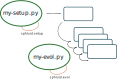
\includegraphics[width=0.8\hsize]{sphluid-arch}
                \caption{
                    Current design for \sphluid architecture.
                }
            \end{figure}

            Because of efficiency requirements, the libraries will be written
            in Rust, but the simple driver programs will be written in Python,
            that is a far more accessible language (reflecting the different
            audience).
            \vspace*{10pt}

            The same model is repeated for the evolution part, for which only
            the evolution step will be done in Rust, but the rest of the
            management will be Python (and as simple as possible).
        \end{column}
    \end{columns}
\end{frame}

\begin{frame}{Analysis}
    \begin{columns}
        \begin{column}{0.5\textwidth}
            The analysis will be done in Python as well, where all the
            libraries to manage the dumps are already available.

            The custom part of the file format (the dump format, built on top
            of some other standard like netCDF4) will be in
            \texttt{sphluid.io}, and available to reuse also in the analysis
            code.
            \vspace*{10pt}

            The analysis framework will leverage all the huge availability of
            tools in Python:
            \begin{itemize}
                \item data structures: NumPy, Pandas, Xarray
                \item scientific computing: Scipy
                \item notebook programming: Jupyter (Notebook/Lab)
                \item machine learning (why not?): Scikit-Learn, TensorFlow
            \end{itemize}
        \end{column}
        \begin{column}{0.5\textwidth}
            Reusable tools will be collected into another library, this time
            pure Python: \sphlash.

            \begin{center}
                \centericon{github}~\href{https://github.com/AleCandido/sphluid/tree/main/sphlash}{AleCandido/sphluid/sphlash}
            \end{center}

            Also this libraries can accept contributions from a wider audience,
            splitting the contributor role from low-level development (high
            performances or graphics).
        \end{column}
    \end{columns}
\end{frame}


\begin{frame}[standout]
    Thanks for your attention!
\end{frame}

\appendix

\begin{frame}{More simulations details}
    \begin{columns}
        \begin{column}{0.5\textwidth}
            \indent\textsc{\textbf{\Large Planet}}
            \vspace*{5pt}
                
            Possible planets modeled have masses $M_\text{p} = [1, 2, 2.5, 3,
            5] M_\text{j}$ at a distance of $R_\text{p} = 34.5$ from the
            central star.

            Even if, in a previous work, a mass of $5.6 M_\text{j}$ was
            estimated, this is excluded by separate runs, and not discussed any
            further in the paper.
        \end{column}
        \begin{column}{0.5\textwidth}
            \indent\textsc{\textbf{\Large Radiation}}
            \vspace*{5pt}

            In order to model the radiation scattered by the dust, to be
            compared with ALMA observations, the \textsc{mcfost} code is used,
            where each \enquote{cell} is associated to an SPH particle.

            The source of radiation is assumed to be the central star, and the
            DIANA dust model is adopted for the dust opacity.
        \end{column}
    \end{columns}
\end{frame}


\begin{frame}[allowframebreaks]{References}
  \bibliography{talk}
  \bibliographystyle{alpha}
\end{frame}

\end{document}
